\documentclass[12pt]{article}

\usepackage{amsmath}
\usepackage{amssymb}
\usepackage{amsfonts}
\usepackage[style=iso]{datetime2}
\usepackage{graphicx}
\usepackage{float}

\graphicspath{ {./Images/} }


\begin{titlepage}
\title{Calculus I: Review of Inverse Functions}
\author{The Melon Man}
\date{\today}
\end{titlepage}

\renewcommand{\thesection}{\Roman{section}}

\allowdisplaybreaks

\setlength{\parindent}{0pt}
\setlength{\parskip}{1em}

\begin{document}
\maketitle

If we have a function $f(x)$ such that $f(x)=x^2$, we may want to find the inverse of this function.
We denote the inverse of some function with the $-1$ before the opening parentheses.
For instance, the inverse of $f(x)$ would be $f^{-1}(x)$.
This should not be confused with raising the function to the $-1$th power, as that would give us something different.
This may be confusing, especially with the trigonometric functions who have well-known inverses as well as functions that equal them raised to the $-1$th power.

Taking the inverse of a function after taking the function may be thought of reversing what the function did and giving back the original $x$ values.
Thus, if the statement $(f(x) \circ g(x))(x) = (g(x) \circ f(x))(x) = x$ is true, then it would hold that $g(x)$ and $f(x)$ are inverses.
We can actaully use this to verify whether a function is an inverse of another, which we will do later.

In the instance above, we have a specific way of finding the inverse of $f(x)$.
While this example may seem simple and the inverse can be easily inferred, the process would be the same for other functions.
We would write it out as an equation in terms of $x$ and $y$:

\begin{equation}
    y = x^2
\end{equation}

We would then swap the two variables with each other:

\begin{equation}
    x = y^2
\end{equation}

Afterwards, we would solve for $y$:

\begin{equation}
    y = \pm \sqrt{x}
\end{equation}

Note that here, we have two values for $y$.
We may replace $y$ with $f^{-1}(x)$ and get:

\begin{align}
    f^{-1}(x) & = \sqrt{x}  \\
              & \&          \\
    f^{-1}(x) & = -\sqrt{x}
\end{align}


Now, we were given two inverse functions for $f(x)=x^2$.
This is due to the fact that each inverse function only works for certain intervals of $x$.
$f^{-1}(x)=\sqrt{x}$ is a valid inverse function for $f(x)=x^2$ for $x$ values on the interval $[0, \infty)$.
                For these $x$ values, it holds true that $(\sqrt{x})^2 = \sqrt{(x^2)} = x$, so $(f \circ f^{-1}) = (f^{-1} \circ f) = x$.
                However, if we have something like $x=-1$, it would be true that $(\sqrt{x})^2 = x$ but not that $\sqrt{(x^2)} = x$ since $\sqrt{(-1)^2} = 1$ and $-1 \neq 1$.
                For $x$ values on the interval $(-\infty, 0]$, the inverse function is $f^{-1}(x)=-\sqrt{x}$.
On this interval, it is true that $(-\sqrt{x})^2 = -\sqrt{(x^2)} = x$, so $(f \circ f^{-1}) = (f^{-1} \circ f) = x$.
For instance, with $x=-1$, $(-\sqrt{x})^2 = x$ is true and so is $-\sqrt{(x^2)} = x$ as $-\sqrt{(-1)^2} = -1$.

The reason $f(x)=x^2$ has multiple inverse functions is because it is not injective.
If a function is injective, then for any value of $f(x)$, there is only one value of $x$ corresponds to it.
$x^2$ is not injectie as $(-x)^2 = x^2$ for all $x \in \mathbb{R}$.
Say we have $f(x) = 4$; it could be true that $x=2$ or $x=-2$.
$\sqrt{(x^2)}$ will return $|x|$ instead of $x$, so $f^{-1}(x)=\sqrt{x}$ does not work as an inverse function for $x<0$ as $(f^{-1} \circ f)$ would not return $x$.
Thus, the function has two inverses that work for different intervals.

Let's try some examples of finding inverse functions:

\begin{enumerate}
    \item $f(x) = 6x + 15$
    \item $h(x) = 3 - 29x$
    \item $R(x) = x^3 + 6$
    \item $g(x) = 4(x-3)^5 + 21$
    \item $W(x) = \sqrt[5]{9-11x}$
    \item $f(x) = \sqrt[7]{5x+8}$
    \item $h(x) = \displaystyle \frac{1+9x}{4-x}$
    \item $f(x) = \displaystyle \frac{6-10x}{8x+7}$
\end{enumerate}

The first one is simple.
The answer is:

\begin{equation}
    f^{-1}(x) = \frac{x-15}{6}
\end{equation}

The second one is:

\begin{equation}
    h^{-1}(x) = \frac{3-x}{29}
\end{equation}

The third one is:

\begin{equation}
    R^{-1}(x) = \sqrt[3]{x-6}
\end{equation}

The fourth one is:

\begin{equation}
    g^{-1}(x) = \sqrt[5]{\frac{x-21}{4}}+3
\end{equation}

The fifth one is:

\begin{equation}
    W^{-1}(x) = \frac{9-x^5}{11}
\end{equation}

The sixth one is:

\begin{equation}
    f^{-1}(x) = \frac{x^7-8}{5}
\end{equation}

The seventh one takes a few more steps.
Let's do it step-by-step:

\begin{align}
    h(x)      & = \frac{1+9x}{4-x} \\
    y         & = \frac{1+9x}{4-x} \\
    x         & = \frac{1+9y}{4-y} \\
    x(4-y)    & = 1+9y             \\
    4x - xy   & = 1+9y             \\
    -xy       & = 1+9y-4x          \\
    xy        & = 4x-1-9y          \\
    xy+9y     & = 4x-1             \\
    y(x+9)    & = 4x-1             \\
    y         & = \frac{4x-1}{x+9} \\
    h^{-1}(x) & = \frac{4x-1}{x+9}
\end{align}

To double check our answer, let's do the composition $(h \circ h^{-1})$ and see if we get $x$ back.

\begin{align}
    (h \circ h^{-1}) & = \frac{1+9(h^{-1})}{4-(h^{-1})}                                                                                                    \\
                     & = \frac{1+9\left(\frac{4x-1}{x+9}\right)}{4-\left(\frac{4x-1}{x+9}\right)}                                                          \\
                     & = \frac{1+\left(\frac{36x-9}{x+9}\right)}{4-\left(\frac{4x-1}{x+9}\right)}                                                          \\
                     & = \frac{\left(\frac{x+9}{x+9}\right)+\left(\frac{36x-9}{x+9}\right)}{\left(\frac{4(x+9)}{x+9}\right)-\left(\frac{4x-1}{x+9}\right)} \\
                     & = \frac{\left(\frac{36x-9+x+9}{x+9}\right)}{\left(\frac{4x+36-4x+1}{x+9}\right)}                                                    \\
                     & = \frac{\left(\frac{37x}{x+9}\right)}{\left(\frac{37}{x+9}\right)}                                                                  \\
                     & = \frac{37x}{x+9} \cdot \frac{x+9}{37}                                                                                              \\
                     & = x
\end{align}

For the last one, we will do the same as before:

\begin{align}
    f(x)       & = \frac{6-10x}{8x+7}   \\
    y          & = \frac{6-10x}{8x+7}   \\
    x          & = \frac{6-10y}{8y+7}   \\
    x(8y+7)    & = 6-10y                \\
    8xy + 7x   & = 6-10y                \\
    8xy + 10y  & = 6-7x                 \\
    y(8x + 10) & = 6-7x                 \\
    y          & = \frac{6-7x}{8x + 10} \\
    f^{-1}(x)  & = \frac{6-7x}{8x + 10}
\end{align}

Now, we could check our answer but the calculations were rather simple so it's safe to assume that is correct.

One other thing which we may show is what inverse functions represent graphically.
The line created by an inverse function will be the original function mirrored along the line $y=x$.
We can see this with the following example:

\begin{figure}[H]
    \centering
    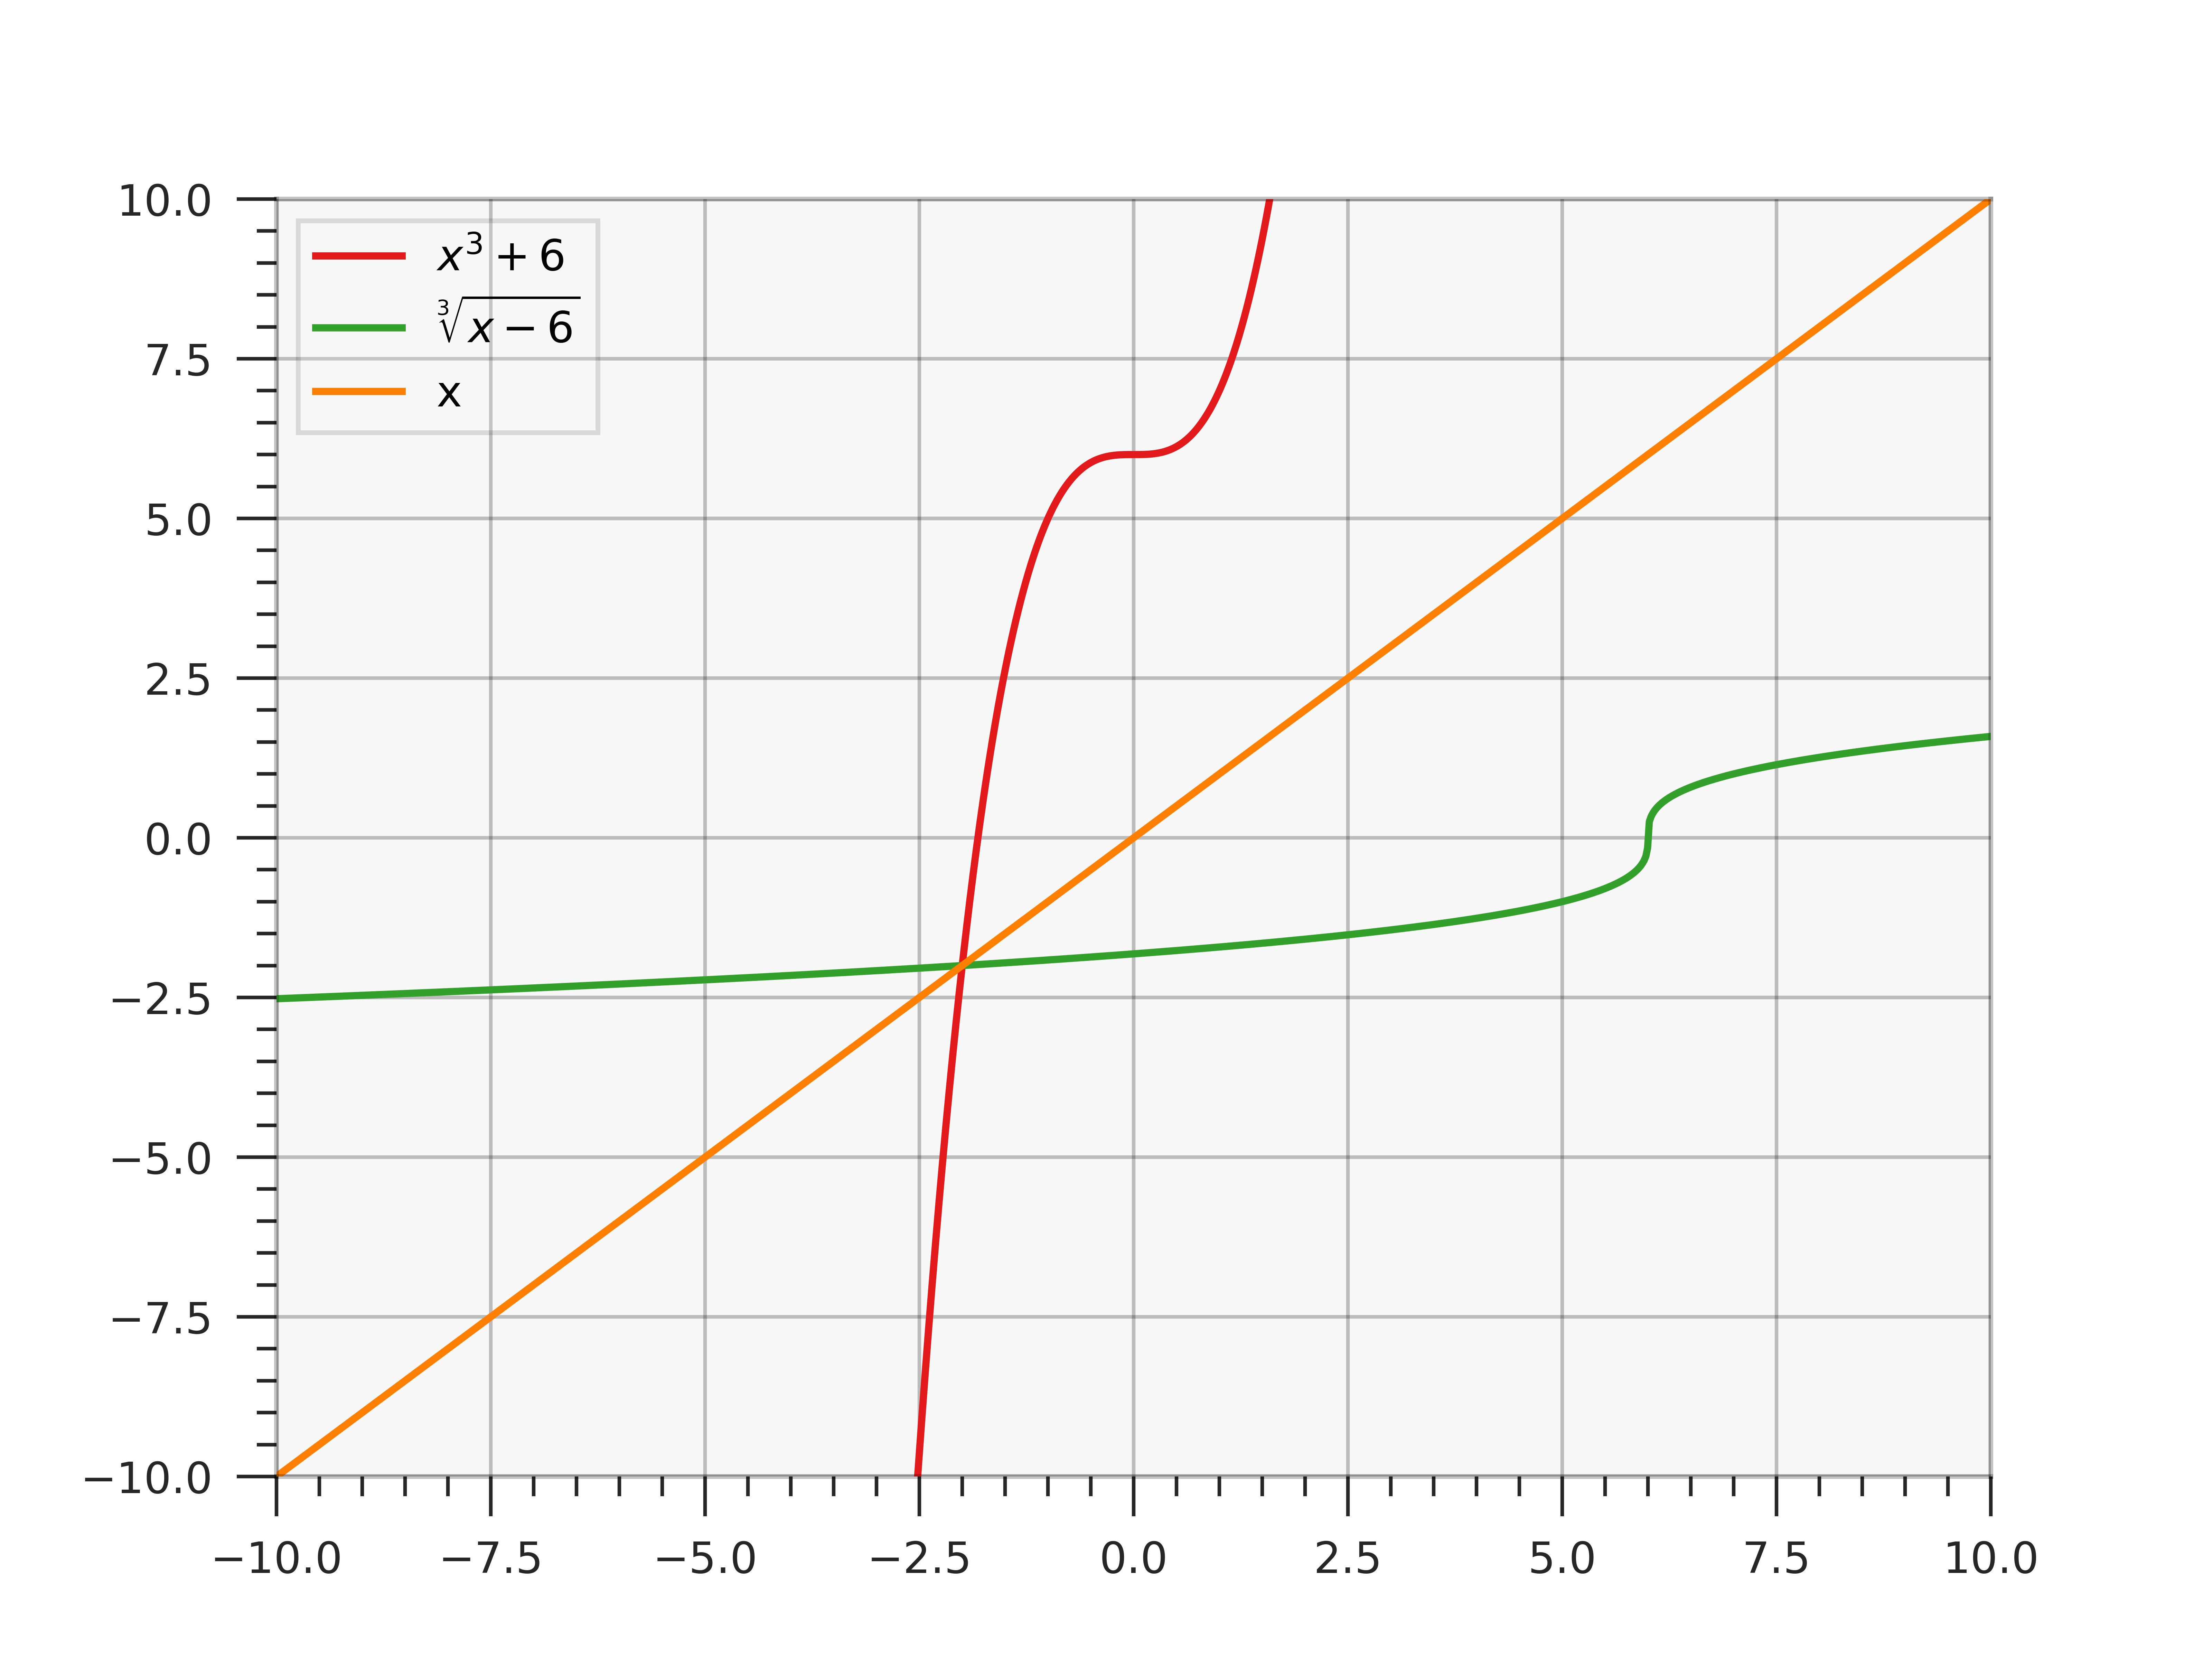
\includegraphics[width=12.5cm, height=10cm]{inverse_functions.png}
    \caption{Inverse Functions}
    \label{fig:fig1}
\end{figure}

This relation between inverse functions will be true for any $f(x)$ and $f^{-1}(x)$.
Even with functions that are not one-to-one, there will be this symmetry for some interval where the function does happen to be one-to-one.
For instance, the function $\sin(x)$ is mirrored with $\arcsin(x)$ in the interval $[-\pi, \pi]$, before the function repeats its $y$ values.

\end{document}